\subsubsection{Security of Suffix Proofs} \label{proof_under_hard_fork}
In this section we provide the full security proof for the NIPoPoWs suffix proof
protocol\cite{nipopows}. Apart from the proof itself (Theorem 2), we describe the
definitions and lemmas being used. We try to give intuition for arguments and
conclusions in each step.

Assume $t$ adversarial out of $n$ total parties, each with $q$ PoW random oracle
queries per round. We define $p = \frac{T}{2^\kappa}$ the probability of a
successful Random Oracle query. We will call a query to the RO $\mu$\textit{-successful}
if the RO returns a value $h$ such that $h \leq 2^{-\mu}T$.

We define the boolean random variables $X_r^{\mu}$, $Y_r^{\mu}$, $Z_r^{\mu}$.
Fix some round $r$, query index $j$ and adversarial party index $k$ (out of $t$).
If at round $r$ an honest party obtains a PoW with $id < 2^{-\mu}T$, set $X_r^{\mu} = 1$,
otherwise $X_r^{\mu} = 0$. If at round $r$ exactly one honest party obtains
$id < 2^{-\mu}T$, set $Y_r^{\mu} = 1$, otherwise $Y_r^{\mu} = 0$. If at round $
r$ the $j$-th query of the $k$-th corrupted party is $\mu$-successful, set
$Z_{rjk}^{\mu} = 1$, otherwise $Z_{rjk}^{\mu} = 0$. Let $Z_r^{\mu} =
\sum_{k=1}^t\sum_{j=1}^qZ_{rjk}^{\mu}$. For a set of rounds $S$, let
$X^\mu(S) = \sum_{r \in S}X^{\mu}_r$ and similarly define $Y_S^{\mu}$, $Z_S^{\mu}$.\\

\begin{defn}[Typical Execution]
	An execution of the protocol is $(\epsilon, \eta)$-typical if:
	
	\textbf{Block counts don't deviate.} For all $\mu \geq 0$ and any set
	$S$ of consecutive rounds with $\vert S \vert \geq 2^\mu \eta k$, we have:
	\begin{itemize}
		\item[-] $(1-\epsilon)E[X^\mu(S)] < X^\mu(S) < (1+\epsilon)E[X^\mu(S)] $ and
			$(1-\epsilon)E[Y^\mu(S)] < Y^\mu(S)$
		\item[-] $Z^\mu(S) < (1+\epsilon)E[Z^\mu(S)]$
\end{itemize}

	\textbf{Round count doesn't deviate.} Let $S$ be a set of consecutive rounds
	such that $Z^\mu(S) \geq k$ for some security parameter $k$. Then $\vert S \vert
	\geq (1-\epsilon)2^\mu \frac{k}{pqt}$ with overwhelming probability.
	
	\textbf{Chain regularity.} No insertions, no copies and no predictions
	\cite{backbone} have occurred.
	\label{defn:typical_execution}
\end{defn}

\begin{thm}[Typicality]
	Executions are $(\epsilon, \eta)$-typical with overwhelming probability in $k$.
\end{thm}
\begin{proof}
	\textbf{Block counts and regularity.} We refer to \cite{backbone} for
	the full proof.

	\textbf{Round count.} First, observe that for a specific round $r$ we have $Z_{rjk}
	\sim Bern(p)$, so for the $\mu$-level superblocks $Z_{rjk}^\mu \sim Bern(2^{-\mu}p)$
	and these are jointly independent. Therefore, since for $\vert S \vert$ rounds we
	have $tq\vert S \vert$ adversarial RO queries, we have that $Z_S^\mu \sim
	\text{Bin}(tq \vert S \vert, 2^{-\mu}p)$. So $tq \vert S \vert \sim
	\text{NB}(Z_S^\mu, 2^{-\mu}p)$. Negative Binomial distribution is defined
	as $\text{NB}(r, p')$ and expresses the number of trials in a sequence of
	independent and identically distributed Bernoulli trials before a specified
	$(r)$ number of successes occurs. The expected total number of trials of a
	negative binomial distribution with parameters $(r, p')$ is $r/p'$. To see
	this, imagine an experiment simulating the negative binomial performed many
	times, that is a set of trials is performed until $r$ successes occur. Consider
	you perform $n$ experiments of total $N$ trials. Now we would expect $Np' = nr$,
	so $N/n = r/p'$. See that $N/n$ is just the average number of trials per
	experiment. So we have $E[tq \vert S \vert] = \frac{Z^\mu_S}{2^{-\mu}p}
	\Rightarrow E[\vert S \vert] = 2^\mu \frac{Z^\mu_S}{tqp}$. So if $Z^\mu(S) \geq k$
	then $E[\vert S \vert] \geq 2^\mu \frac{k}{tqp}$. Applying a tail bound to the
	negative binomial distribution, we obtain that $\text{Pr}[\vert S \vert < (1 -
	\epsilon)E(\vert S \vert)] \in \Omega(\epsilon^{2}m)$.
\end{proof}

\begin{lemma}
	Suppose S is a set of consecutive rounds $r_1 ... r_2$
	and $C_B$ is a chain adopted by an honest party at round $r_2$ of a typical
	execution. Let $C^{B}_{S} = \{$ b $\in C_B:$ b was generated during $S\}$. Let
	$\mu_A, \mu_B \in \mathbb{N}$. Suppose $C^{B}_{S}\uparrow^{\mu_B}$ is good.
	Suppose $C'_A$ is a $\mu_A$-superchain containing only adversarially generated
	blocks generated during S and suppose that $\vert C'_A \vert \geq k$. Then
	$2^{\mu_A} \vert C'_A \vert <  2^{\mu_B} \vert    C^{B}_{S}\uparrow^{\mu_B}\vert $.
	\label{lemma:honest_vs_pure_adversarial_subchain}
\end{lemma}
\begin{proof}
	From $\vert C'_A \vert \geq k$ we have that $\vert Z^{\mu_A}_S
	\vert \geq k$. Applying Theorem 1, we conclude that $\vert S \vert \geq
	(1-\epsilon')2^{\mu_A} \frac{\vert C'_A \vert}{pqt}$. Applying the Chain Growth
	theorem \cite{backbone} we obtain $\vert C_{B}^S \vert \geq (1 - \epsilon)f
	\vert S \vert$. But from the goodness of $C_{B}^S \uparrow^{\mu_B}$, we know
	that $\vert C_{B}^S\uparrow^{\mu_B} \vert \geq (1 - \delta)2^{-\mu_B} \vert
	C_{B}^S \vert $. So we have $\vert C_{B}^S\uparrow^{\mu_B} \vert \geq
	(1 - \delta)2^{-\mu_B} (1 - \epsilon)f \vert S \vert $ and follows that
	$\vert C_{B}^S\uparrow^{\mu_B} \vert \geq (1 - \delta)2^{-\mu_B} (1 - \epsilon)f
	(1-\epsilon')2^{\mu_A} \frac{\vert C'_A \vert}{pqt} $. Consequently we have that
	$2^{\mu_A} \vert C'_A \vert \leq \frac{pqt}{(1- \delta)(1-\epsilon)(1-\epsilon')f}
	2^{\mu_B} \vert C_{B}^S\uparrow^{\mu_B} \vert $.   \\

	So, according to the above equation we have that $2^{\mu_A} \vert C'_A \vert
	<  2^{\mu_B} \vert    C^{B}_{S}\uparrow^{\mu_B}\vert $ considering that honest
	majority assumption holds, specifically considering that $ \frac{pqt}{f} \approx
	\frac{t}{n-t} \leq 1 $ .
\end{proof}

\begin{defn}[Adequate level of honest proof]
	Let $\pi$ be an
	honestly generated proof constructed upon some adopted chain $C$ and let $b \in 
	\pi $. Then $\mu'$ is defined as $\mu' = \max \{ \mu: \vert \pi\{b:\}\uparrow^{\mu}
	\vert \geq \max( m+1, (1-\delta)2^{-\mu} \vert \pi\{b:\}\uparrow^{\mu}\downarrow \vert )\}$.
	We call $\mu'$ the adequate level of proof $\pi$ with respect to block b with
	security parameters $\delta$ and m. Note that the adequate level of a proof is a
	function of both the proof $\pi$ and the chosen block b.
\end{defn}

Intuitively, adequate is the level $\mu'$ of a proof $\pi$ for a block b
if there are at least $m$ blocks after b in $\pi$ under the condition that there
is good chain quality for this level, meaning that there are at least so many blocks
at this level as expected considering the number of 0-level blocks.\\
NOTE: adequate level is mostly useful for Claim 1a of the Security Proof (Theorem 2).\\

\begin{lemma}
	Let $\pi$ be some honest proof generated with security
	parameters $\delta$, m. Let C be the underlying chain, $b \in C$ be any block
	and $\mu'$ be the adequate level of the proof with respect to b and the same
	security parameters.\\Then $C\{b:\}\uparrow^{\mu'} = \pi\{b:\}\uparrow^{\mu'}$.
	\label{lemm:complete_adequate}
\end{lemma}
\begin{proof}
	$ \pi\{b:\}\uparrow^{\mu'} \subseteq C\{b:\}\uparrow^{\mu'}$ is
	trivial. For the converse, we have that in the iteration of the \emph{Prove for
	loop}\cite{nipopows} with $\mu = \mu^*$, the block stored in variable $B$
	precedes $b$ in $C$.

	Note that the Prover's for loop iterates over all levels in the interlink structure,
	and places in the proof all of the blocks that are of the corresponding level and succeed $B$ in $C$.

	Suppose $\mu = \mu^*$ is the first \emph{for} iteration during which the property
	is violated. This cannot be the first iteration since $B = C[0]$ and Genesis
	precedes all blocks. By induction hypothesis we see that during the iteration
	$\mu = mu^* + 1$, $B$ preceded $b$. From the definition of $\mu'$ we know that
	$\mu'$ is the highest level for which $\vert \pi\{b:\}\uparrow^{\mu} \vert
	\geq \max( m, (1-\delta)2^{-\mu} \vert \pi\{b:\}\uparrow^{\mu}\downarrow \vert ) $.

	Hence, this property cannot hold for $\mu^* > \mu$ and therefore $\vert
	\pi\{b:\}\uparrow^{\mu} \vert < m$ or $\neg$local-good$_\delta(\pi\{b:
	\}\uparrow \mu^*[1:], C, \mu^*)$.

	In case local-good is violated, variable $B$ remains unmodified and the induction
	step holds. If local-good is not violated, then $ \vert \pi\{b:\} \uparrow^{\mu^*}[1:]
	\vert < m$ and so $\pi\uparrow^{\mu^*}[-m]$, which is the updated value of $B$ at the
	end of $\mu^*$ iteration, precedes $b$.
\end{proof}

\begin{lemma}
	Suppose the verifier evaluates $\pi_A \geq \pi_B$ in a
	protocol interaction where B is honest and assume during the comparison that the
	compared level of the honest party is $\mu_B$. Let $b = LCA(\pi_A, \pi_B)$ and
	let ${\mu}'_B$ be the adequate level of $\pi_B$ with respect to b. Then ${\mu}'_B
	\geq \mu_B$.
	\label{lemm:greatest_adequate}
\end{lemma}
\begin{proof}
	Because $\mu_B$ is the compared level of the honest party, from
	the definition of the $\geq_m$ operator, we have $2^{\mu_B} \vert \pi\{b:\}\uparrow^{\mu_B}
	\vert > 2^{{\mu}'_B} \vert \pi\{b:\}\uparrow^{{\mu}'_B} \vert $. This is true,
	otherwise the Verifier would have chosen level $\mu'_B$ as level of comparison.
	The proof is by contradiction. Suppose $\mu'_B < \mu_B$.
	By definition, $\mu'_B$ is the maximum level such that $\vert \pi_B\{b:\}\uparrow^\mu
	[1:] \vert \geq max(m, (1-\delta)2^{-\mu}\vert \pi_B\{b:\}\uparrow^\mu [1:]\downarrow
	\vert)$, therefore $\mu_B$ does not satisfy this condition.
	But we know that $\vert \pi_B\{b:\}\uparrow^\mu [1:] \vert > m$ because
	$\mu_B$ was selected by the Verifier.
	Therefore $ 2^{\mu_B} \vert \pi\{b:\}\uparrow^{\mu_B} \vert < (1-\delta)\vert
	C\{b:\}\vert $. \\
	But also $\mu'_B$ satisfies goodness, so $ 2^{\mu'_B} \vert \pi\{b:\}\uparrow^{\mu'_B}
	\vert > (1-\delta)\vert C\{b:\}\vert $.\\ From the last two equations we obtain
	$ 2^{\mu_B} \vert \pi\{b:\}\uparrow^{\mu_B} \vert < 2^{\mu'_B} \vert
	\pi\{b:\}\uparrow^{\mu'_B} \vert$ which contradicts the initial equation.
\end{proof}

Intuitively the above Lemma says: the comparison level chosen by the Verifier can be
no other than the adequate level in respect to block b ($LCA(\pi_A, \pi_B)$), since
any other choice would be a level of non-good quality, because of the definition of
the adequate level. A level of non-good quality would contain less PoW than that of
the adequate level for the range of interest $C\{b:\}$. \\

\begin{thm}[Security of suffix proofs]
	Assuming honest majority, the non-interactive
	proofs-of-proof-of-work construction for computable $\kappa$-stable monotonic
	suffix-sensitive predicates is secure with overwhelming probability in $\kappa$.
	\label{thm:original_suffix_security}
\end{thm}
\begin{proof}
	By contradiction. Let $Q$ be a $\kappa-$stable monotonic
	suffix-sensitive chain predicate. Assume NIPoPoWs on $Q$ is insecure. Then,
	during an execution at some round  $r_3$, $Q(C)$ is defined and the verifier
	$V$ disagrees with some honest participant. Assume the execution is typical.
	$V$ communicates with adversary $A$ and honest prover $B$. The verifier receives
	proofs $\pi_A, \pi_B$. Because $B$ is honest, $\pi_B$ is a proof constructed
	based on underlying blockchain $C_B$ (with $\pi_B \subseteq C_B$), which $B$
	has adopted during round $r_3$ at which $\pi_B$ was generated. Furthermore,
	$\pi_A$ was generated at round $r'_3 \leq r_3$.

	The verifier outputs $\neg Q(C_B)$. Thus it is necessary that $\pi_A \geq 
	\pi_B$. We will show that this is a negligible event.

	Let $b = LCA(\pi_A, \pi_B)$. Let $b^\star$ be the most recently honestly
	generated block in $C_B$ preceding $b$. Note that $b^\star$ necessarily
	exists because Genesis is honestly generated. Let the levels of comparison
	decided by the verifier be $\mu_A$ and $\mu_B$ respectively. Let $\mu'_B$
	be the adequate level of proof $\pi_B$  with respect to block $b$. Call
	$\alpha_A = \pi_A \uparrow^{\mu_A}\{b:\}$,
	$\alpha'_B = \pi_B \uparrow^{\mu'_B}\{b:\}$.

	%%ANDRI:
	Note that we consider the parts of the proofs succeeding block $b$ the decisive ones 
	for the verifier's choice. This is to adversary's advantage, since the parts 
	preceding this block demonstrate the proof-of-work contained in the common 
	(sub)chain, thus the adversary could only include equal or less proof-of-work
	in her proof for this part of the chain.

	We will now show three successive claims: First, $\alpha_A$ and $\alpha'_B \downarrow$
	are mostly disjoint. Second, $a_A$ contains mostly adversarially generated blocks.
	And third, the adversary is able to produce this $a_A$ with negligible probability.

	Let $\alpha_A = k_1 + k_2 + k_3$ and let $k_1, k_2, k_3$ be as defined in the
	following Claims.

	\textbf{Claim 1:} $\alpha_A, \alpha'_B\downarrow$ are mostly disjoint. We show
	this by taking the two possible cases for the relation of $\mu_A$, $\mu'_B$.\\
	\textit{\underline{Claim 1a}:} If $\mu'_B \leq \mu_A$ then they are completely
	disjoint. In such a case of inequality, every block in $\alpha_A$ would also be
	of lower level $\mu'_B$. Applying Lemma 2 to $C\{b:\}\uparrow^{\mu'_B}$  we see
	that $C\{b:\}\uparrow^{\mu'_B} = \pi\{b:\}\uparrow^{\mu'_B}$. Subsequently, any
	block in $\pi_A\uparrow^{\mu_A}\{b:\}[1:]$ would also be included in proof
	$\alpha'_B$, but $b=LCA(\pi_A, \pi_B)$ so there can be no succeeding block
	common in $\alpha_A, \alpha'_B$. \\
	\\
	\textit{\underline{Claim 1b}:} If  $\mu'_B > \mu_A$ then $\vert \alpha_A[1:] 
	\cap \alpha'_B\downarrow[1:] \vert = k_1 \leq 2^{\mu'_B - \mu_A}$.\\
	%% possibly unnecessary sentence%%%%%
	First observe that because the adversary is winning $2^{\mu_A} \vert \alpha_A \vert 
	> 2^{\mu'_B} \vert \alpha'_B \vert \geq 2^{\mu'_B} m \Rightarrow \vert \alpha_A \vert 
	> 2^{\mu'_B - \mu_A}m$.
	%%%%%%%%%%%%%%%%%%%%%%%%%%%%%%%%%%%%%%%%%%
	Let's call $b_1$ the first block in $\alpha'_B$ after block b.
	Suppose for contradiction that $k_1 > 2^{\mu'_B - \mu_A}$.  Since $C_B^{\mu'_B}$ is
	of good chain quality, this would mean that block $b_1$, of level $\mu'_B$ is also
	of level $\mu_A$. Since it is of level $\mu_A$ the adversary could include it in
	the proof but $b_1$ cannot exist in both $\alpha_A, \alpha'_B$ since $\alpha_A
	\cap \alpha'_B = \emptyset$ by definition. In case that the adversary chooses not
	to include $b_1$ in the proof then she can include no other blocks of $C_B$ in
	her proof, since it would not consist a valid chain.  \\


	From Claim $1a$ and Claim $1b$, we conclude that there are $\vert \alpha_A
	\vert - k_1$ blocks after block $b$ in $\alpha_A$ which do not exist in
	$\alpha_B\downarrow$. We now set $b_2 = LCA(C_B, \alpha_A)$. This makes $b_2$
	the last block before the fork point at the 0-level chain included in the adversary's proof.\\

	Intuition: in this case the common blocks of $\alpha_A, \alpha'_B\downarrow$
	may only be blocks of level $\mu_A$ which precede the first $\mu'_B$ block
	appearing in $\alpha'_B$. If this block of level $\mu'_B$ was common, it could
	also be included in $\alpha_A$. If it is included this would be the LCA of
	$\alpha_A, \alpha'_B$. If it is not, then the adversary could no more include
	blocks from the common part of chain $C_B$ in her proof since they no longer
	form a valid chain in $\alpha_A$. The quantity $2^{\mu'_B - \mu_A}$ means: in
	the range between two consequent $\mu'_B$-level blocks, we have $n = 2^{\mu'_B}$
	0-level blocks and, thus, $2^{-\mu_A}n = 2^{\mu'_B - \mu_A}$ blocks of $\mu_A$-level. \\

	\textbf{Claim 2:} At least $k_3$ superblocks of $\alpha_A$ are adversarially generated.
	We show this by showing that $\alpha_A[k_1 + k_2 + 1:]$ contains no honestly generated
	blocks. Suppose for contradiction that the block $\alpha_A[i]$ for some $i \geq k_1 +
	k_2 + 1$ was honestly generated. This means that an honest party adopted the chain
	$\alpha_A[:i - 1]\downarrow$ at some round $r_2 \leq r_3$. Because of the way honest
	parties adopt chains, the superchain $\alpha_A[:i - 1]$ has an underlying properly
	constructed 0-level anchored chain $C_A$ such that $\alpha_A[:i - 1] \subseteq C_A$.
	Let $j$ be the index of block $b_2$ within $\alpha_A$, $j_\downarrow$ be the index
	of block $b_2$ within $C_A$ and $k_{2\downarrow} = \vert \alpha_A[j:j+k_2]\downarrow\vert$.
	See Figure \ref{fig:proof} for a demonstration. Observe that $\vert C_A[:\{\alpha_A[i-1]\}]
	\vert \geq \vert C_A[:{j_\downarrow}+k_{2\downarrow}] \vert$, while
	$C_A[j_\downarrow:j_\downarrow + k_{2\downarrow}] \npreceq C_B$ as proved in
	Claim 1. But $C_A$ was adopted by an honest party at round $r_2$, which is prior
	to round $r_3$ during which $C_B$ was adopted by an honest party B. This 
	contradicts the Common Prefix\cite{backbone} with parameter $k_{2\downarrow}$. I
	t follows that with overwhelming probability in $k_{2\downarrow}$, the $k_3 =
	\vert \alpha_A \vert - k_2 - k_1$ last blocks of the adversarial proof have
	been adversarially generated.\\

	\begin{figure}[h]
		\begin{center}
			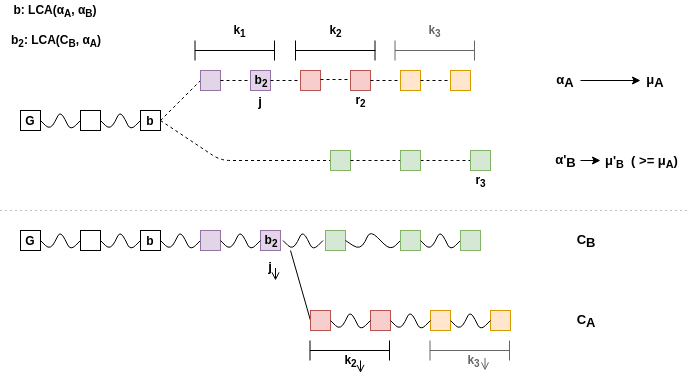
\includegraphics[width=0.9\columnwidth]{figures/proof.png}
		\end{center}
		\caption{Two competing proofs at different levels. At the bottom the
		corresponding 0-level chains are represented.}
		\label{fig:proof}
	\end{figure}

	Intuition: Because of Common Prefix on $k_{2\downarrow}$ parameter, where
	$k_{2\downarrow} = \vert \alpha_A[j:j+k_2]\downarrow\vert$, where
	$E[k_{2\downarrow}] = 2^{\mu_A}k_2$, there can be no honest party adopting
	$C_A$ at any round $i \geq k_1 + k_2 + 1$. \\

	From these two Claims we have that $k_1$ blocks in $\alpha_A$ are blocks of the
	common zero-level chain, while $k_2$ blocks are blocks after the fork point at
	the zero-level chain. Subsequently, $k_2$ is subject to the Common Prefix
	$\kappa-$parameter limitations as described in the Backbone paper\cite{backbone}.\\

	\textbf{Claim 3:} Adversary $A$ is able to produce $\alpha_A$ that wins against
	$\alpha_B$ with negligible probability.

	Let $b'$ be the latest honestly generated block in $a_A$, or $b' = b^*$ if no
	such block exists in $a_A$. Let $r_1$ be the round when $b'$ was generated.
	Consider the set $S$ of consecutive rounds $r_1..r_3$. Every block in
	$\alpha_A[-k_3:]$ has been adversarially generated during $S$ and $\vert
	\alpha_A[-k_3:] \vert = \vert \alpha_A\{b':\} \vert = k_3$. $C_B$ is a chain
	adopted by an honest party at round $r_3$ and filtering the blocks by the rounds
	during which they were generated to obtain $C_B^S$, we see that if $b''$ is the
	most recently generated block in $\alpha_B$ in a round $r \leq r_1$, then $C_B^S =
	C_B\{ b'': \}$. But $C_B^S \uparrow^{\mu'_B}$ is good with respect to $C_B^S$.
	Applying Lemma 1, we obtain that with overwhelming probability  $2^{\mu_A} \vert
	\alpha_A\{b':\} \vert < 2^{\mu'_B} \vert C_B^S \uparrow^{\mu'_B} \vert$, which is
	equal to

	\begin{equation}
	2^{\mu_A} \vert \alpha_A\{b':\} \vert < 2^{\mu'_B} \vert \alpha'_B\{b'':\} \vert
	\end{equation} 

	since $\alpha'_B$ contains all the $\mu'_B$-level blocks in $C_B^S$. \\


	In order to complete the proof, let us now consider $\alpha_A^{k_1}$,
	$\alpha_A^{k_2}$, $\alpha_A^{k_3}$ the parts of $\alpha_A$ where the
	$k_1$, $k_2$, $k_3$ blocks reside and $\alpha_B^{k_1}$, $\alpha_B^{k_2}$,
	$\alpha_B^{k_3}$ the parts of $\alpha_B$ containing blocks generated in the
	corresponding round sets as illustrated in Figure \ref{fig:claim3}.

	\begin{figure}[h]
		\begin{center}
			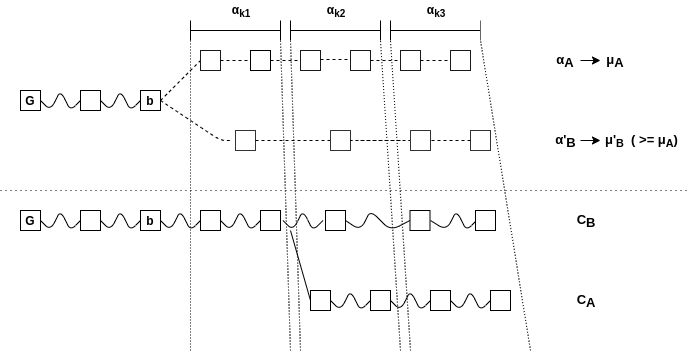
\includegraphics[width=0.9\columnwidth]{figures/claim3.png}
		\end{center}
		\caption{The three round sets in two competing proofs at different levels.
		The vertical dashed lines denote the area of interest, across proofs and chains,
		corresponding to each round set. At the bottom the corresponding 0-level chains
		are represented.}
		\label{fig:claim3}
	\end{figure}

	Subsequently to the above Claims we have that:

	Because of the common underlying chain in the first round set:
	\begin{equation} \label{eq_round_set_1}
	2^{\mu_A} \vert \alpha_A^{k_1} \vert \leq 2^{\mu'_B} \vert \alpha'{_B^{k_1}} \vert
	\end{equation}

	Because of the adoption by an honest party of chain $C_B$ at a later round $r_3$, 
	we have for the second round set:
	\begin{equation} \label{eq_round_set_2}
	2^{\mu_A} \vert \alpha_A^{k_2} \vert \leq 2^{\mu'_B} \vert \alpha'{_B^{k_2}} \vert
	\end{equation}

	Because of Equation (1), we have for the third round set:
	\begin{equation} \label{eq_round_set_3}
	2^{\mu_A} \vert \alpha_A^{k_3} \vert < 2^{\mu'_B} \vert \alpha'{_B^{k_3}} \vert
	\end{equation}

	So we have

	\begin{equation*}
	2^{\mu_A} ( \vert \alpha_A^{k_1} \vert + \vert \alpha_A^{k_2} \vert + \vert
	\alpha_A^{k_3} \vert ) < 2^{\mu'_B} ( \vert \alpha'{_B^{k_1}} \vert + \vert
	\alpha'{_B^{k_2}} \vert + \vert \alpha'{_B^{k_3}} \vert)
	\end{equation*}

	and finally
	\begin{equation}
	2^{\mu_A} \vert \alpha_A \vert < 2^{\mu'_B} \vert \alpha'{_B} \vert
	\end{equation}


	Therefore we have proven that $2^{\mu'_B} \vert \pi_B \uparrow^{\mu'_B} \vert >
	2^{\mu_A} \vert \pi_A^{\mu_A} \vert$. From the definition of $\mu_B$, we know
	that $2^{\mu_B} \vert \pi_B \uparrow^{\mu_B} \vert > 2^{\mu'_B} \vert \pi_B
	\uparrow^{\mu'_B} \vert$ because it was chosen $\mu_B$ as level of comparison
	by the Verifier. So we conclude that $2^{\mu_B} \vert \pi_B \uparrow^{\mu_B}
	\vert > 2^{\mu_A} \vert \pi_A \uparrow^{\mu_A} \vert$.

\end{proof}

It remains to calculate the security parameter $m$ that guarantee that all the above
hold true in every implementation. It suffices to compute a security parameter
value for each set of rounds $k_1, k_2, k_3$, so that the proof equations
\ref{eq_round_set_1}, \ref{eq_round_set_2}, \ref{eq_round_set_3} hold and
then sum these values to obtain parameter $m$.

In the first set of rounds, for the first $k_1$ blocks in $\alpha_A$, we only need
one block included in $\alpha_B$ for the part of the proof described in Equation
\ref{eq_round_set_1}. In the second set of rounds we need $2^{-\mu_B}\kappa$ blocks
for the part of the proof described in Equation \ref{eq_round_set_2}, just as it
directly results from the Common Prefix property. In order to make $m$ independent
of any specific level it suffices to consider the upper bound of $\kappa$ blocks
for this set of rounds. In the last set of rounds we need at least $\kappa$
adversarially generated blocks in $\alpha_A^{k_3}$ so that Lemma 1 is applicable.
Since we assume honest majority, obliging to at least $\kappa$ blocks for this
set of rounds suffices to guarantee for Equation \ref{eq_round_set_3}.

So, we finally conclude to the following upper bound for the value of the
security parameter:
\begin{equation}
	m = 2\kappa + 1
\end{equation}